\section{Visión General del Producto}
El sistema se presenta a sus usuarios como una aplicación web única,
accesible desde cualquier dispositivo con navegador, organizada en torno a
los nueve dominios funcionales descritos en la \hyperlink{section2.2}{sección 2.2}. La pantalla de inicio se
adapta al rol y nivel del usuario autenticado, mostrando únicamente las
operaciones para las que está habilitado.
\par
\vspace{5mm}
Para los voluntarios operativos en el centro, la experiencia se concibe como
un panel táctil de operación directa: las acciones más frecuentes (registrar
una ducha, entregar una prenda, anotar una entrada de alimento) son
accesibles en uno o dos toques desde la pantalla principal. 
\par
\vspace{5mm}
Para los voluntarios profesionales, el sistema se presenta como un expediente clínico
o jurídico clásico, con vista de ficha del amigo y formulario de
anotaciones. Para la coordinación y la directiva, el sistema se presenta
como un cuadro de mando con indicadores agregados, accesos a los módulos de
gestión y exportadores de informes.
\par
\vspace{5mm}
La configuración del sistema reside en su totalidad en la base de datos y en
las variables de entorno del entorno de despliegue. No existen ficheros de
configuración locales que el usuario deba editar, lo que garantiza que la
operación cotidiana no requiere conocimientos técnicos.


\subsection{Entorno de Despliegue}
El despliegue se automatiza mediante \textbf{GitHub Actions:} los \texttt{push} a la rama
de producción tras superar las pruebas automatizadas desencadenan la
construcción de las imágenes Docker, su publicación al registro de Render
y el \texttt{rollout} progresivo de las nuevas versiones. El despliegue automático
puede deshabilitarse para producción con el fin de exigir aprobación manual
en releases sensibles.
\par
\vspace{5mm}
Los usuarios acceden al sistema desde tres tipos de dispositivos: tablets
resistentes propiedad del centro durante los turnos operativos, portátiles
personales de la directiva y voluntarios profesionales desde sus
domicilios, y dispositivos móviles para consulta puntual por parte de la
coordinación. Todos ellos requieren un navegador moderno (Chrome, Firefox,
Safari o Edge en sus dos últimas versiones mayores) y conectividad a
Internet.
\par
\vspace{5mm}
El siguiente diagrama de despliegue resume la arquitectura:

\begin{figure}[H]
    \centering
    \caption{Diagrama de despliegue del sistema}
    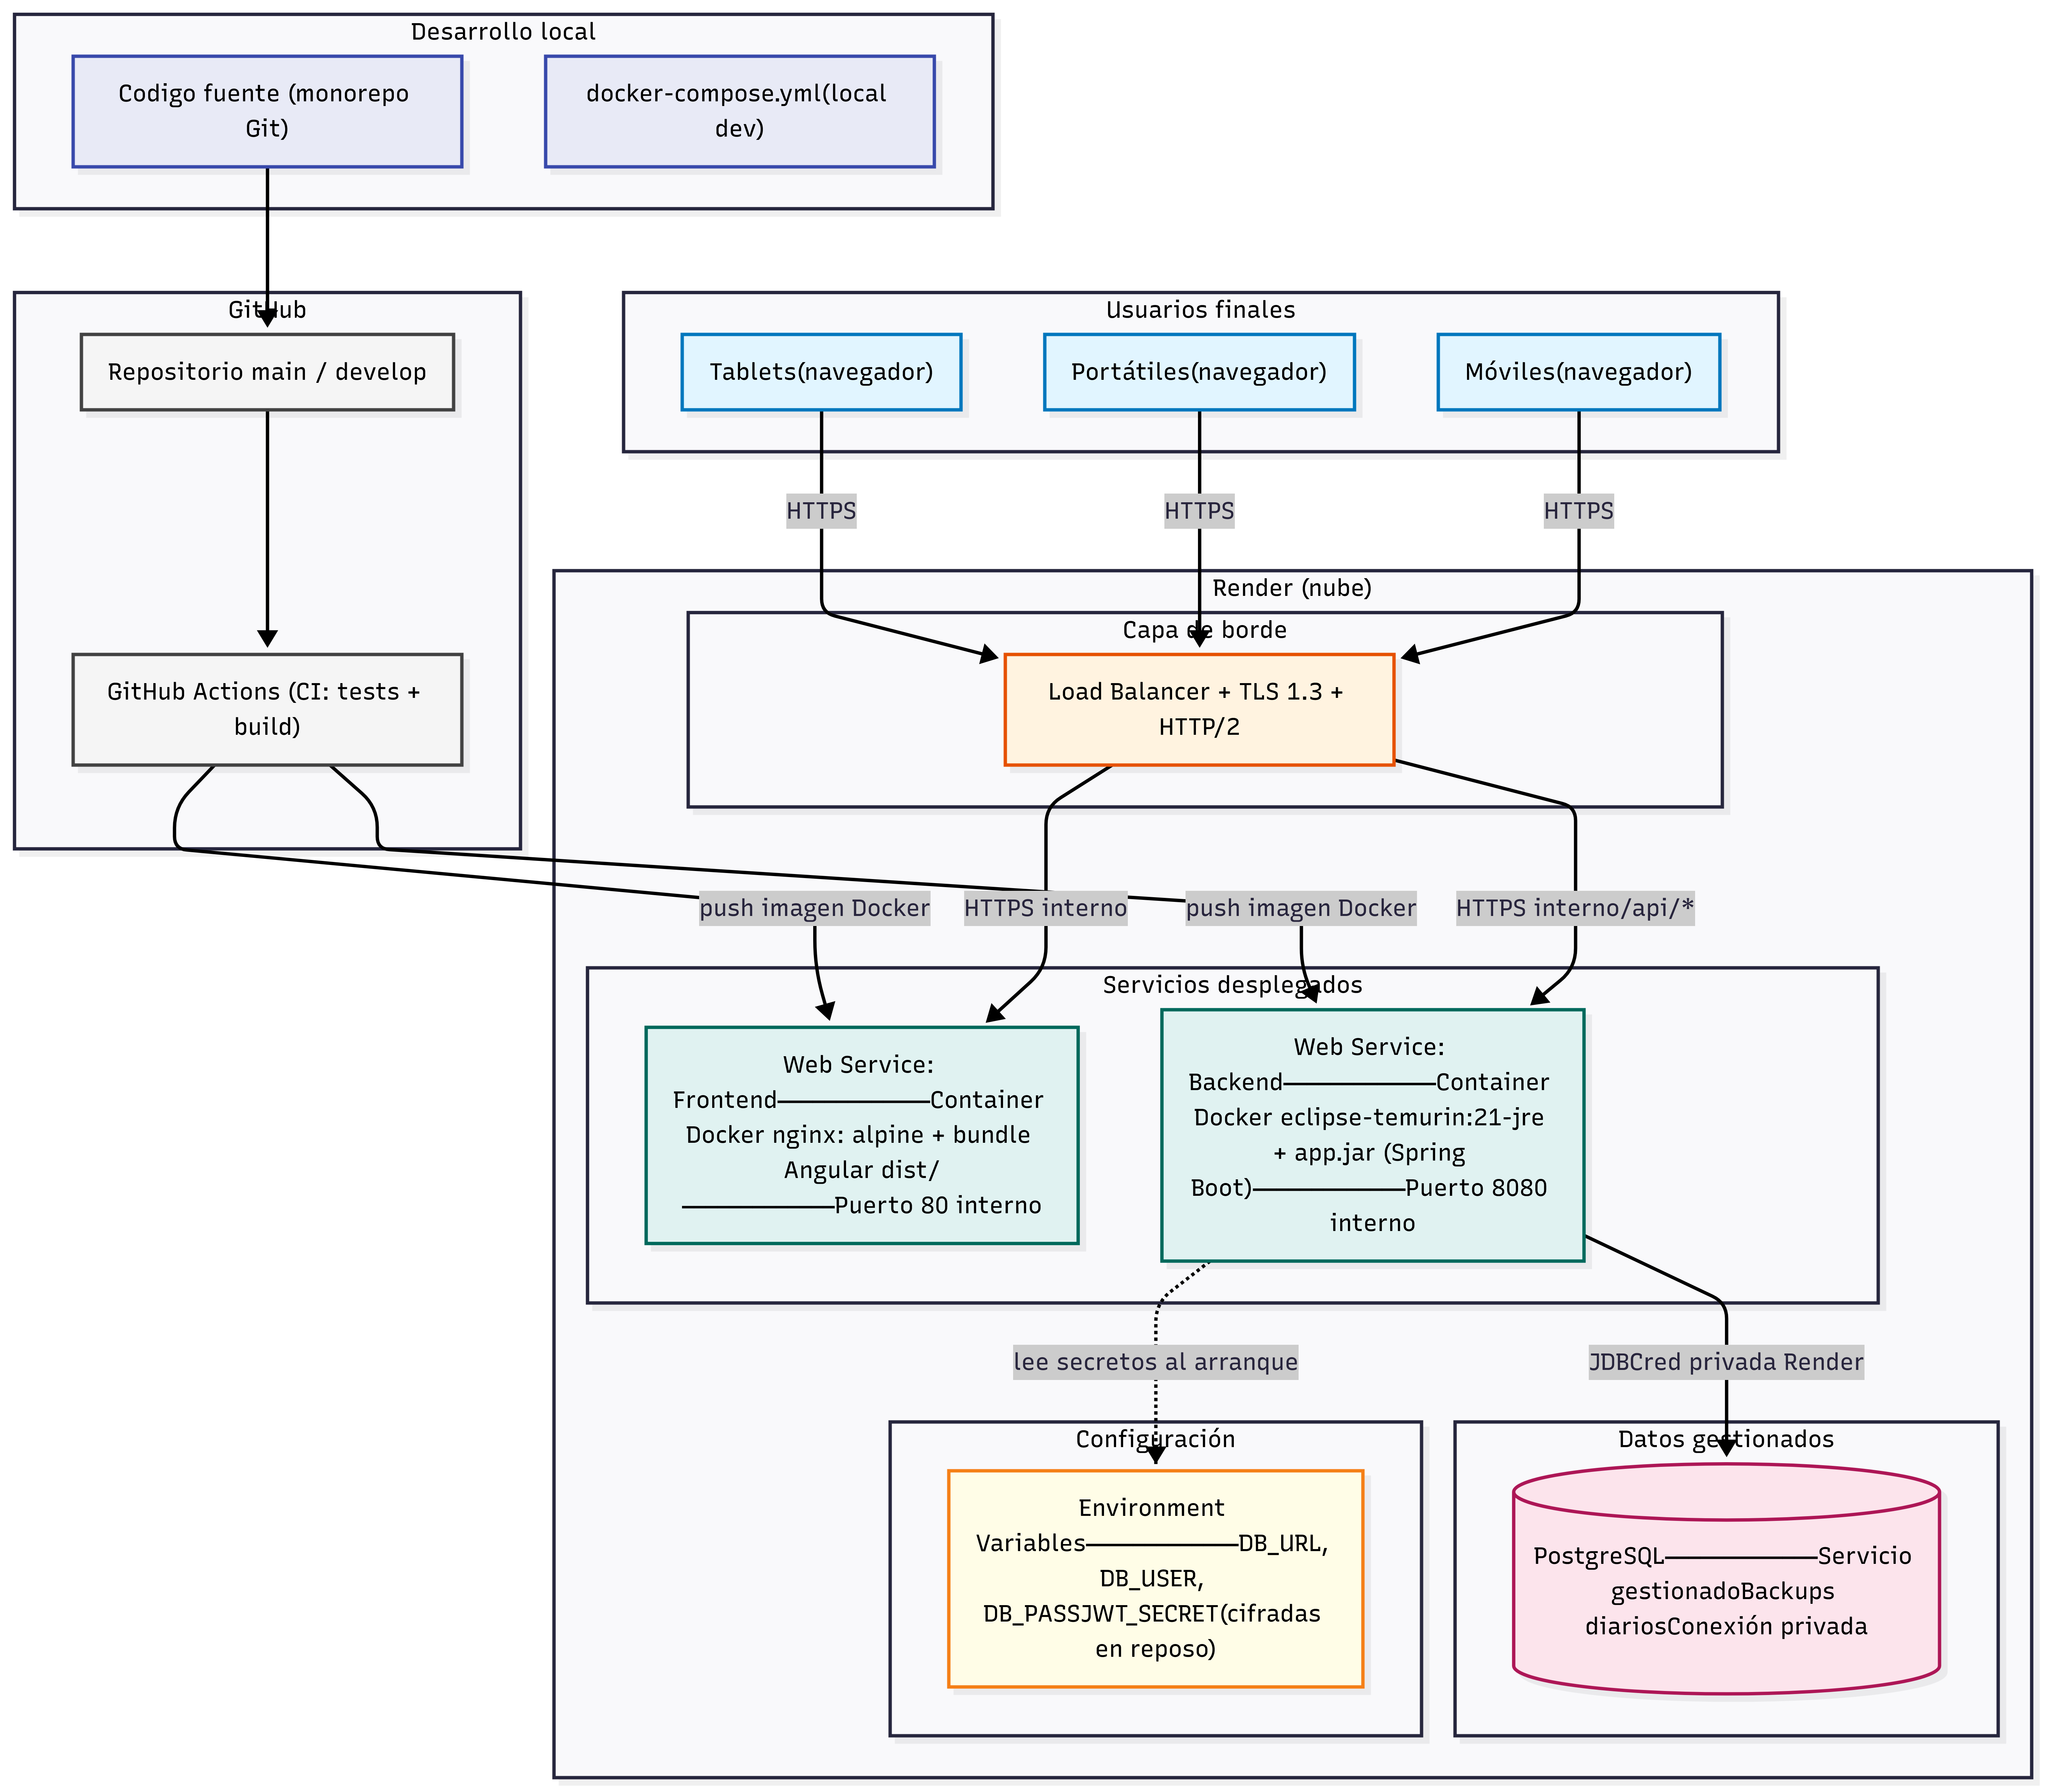
\includegraphics[width=1\linewidth]{assets/mermeid/Diagrama-despliegue-arquitectura.png}
\end{figure}
\par
\vspace{5mm}


\subsubsection{Entorno para la Implementación del Sistema Actual}
El sistema se implementará de forma local usando un proyecto en IntelliJ IDEA, con una base de datos 
PostgreSQL local (montada desde Docker) para desarrollo y pruebas. El entorno de desarrollo se configura mediante Docker Compose, 
que orquesta los contenedores de la aplicación y la base de datos, se harán commits a GitHub desde la misma
máquina donde el repositorio está configurado siguiendo estrategias CI en cada \texttt{pull request}, asi como enfoque tradicional de pruebas 
o TDD donde aplique para asegurar un sistema robusto en cada iteración. En Render se despliegue final cuando el stack backend y frontend haya sido 
previamente probado y optimizado en local. De esta manera, se aprovecha el periodo de 30 días de plan gratuito para someter el sistema completo 
a uso real y finalizar de optimizar lo necesario antes de tener que pagar mensualmente.

\newpage

\subsection{Suposiciones y Dependencias que Asume el Equipo en Torno al Proyecto}
\begin{itemize}
    \item El volumen de amigos atendidos se mantiene en el orden de magnitud
    actual (decenas, sin superar el centenar simultáneo) durante al menos
    los dos primeros años de operación del sistema.

    \item Los requisitos legales de la Ley 1/2025 no sufren modificaciones
    sustantivas durante el periodo de desarrollo. Si se publicaran
    reglamentos de desarrollo o instrucciones técnicas adicionales, sería
    necesario revisar el módulo de trazabilidad alimentaria.

    \item Además de la Ley 1/2025, no hay otras normativas sectoriales 
    (sanitarias, laborales, de protección de datos) que afecten directamente 
    a la operación del sistema. En caso de que se publicaran nuevas normativas, 
    sería necesario revisar el diseño del sistema para garantizar su cumplimiento integrándolo en él.
\end{itemize}


\subsubsection{Factores Externos que Tienen un Efecto en el Producto, pero No son Restricciones Obligatorias}
\begin{itemize}
    \item \textbf{Crecimiento de la asociación.} Si la asociación amplía su radio de
    acción geográfico o incorpora nuevas delegaciones, el modelo de datos
    necesitará incorporar el concepto de ``centro'' o ``delegación'' como
    entidad organizativa.
    
    \item \textbf{Incorporación de nuevas entidades donantes.} La incorporación de
    un nuevo donante con convenio formal podría implicar nuevas
    exigencias documentales, y el sistema no debería tener problemas para adaptarse.
    
    \item \textbf{Incremento en el precio sobre los planes de Render.} Si el coste de
    los planes contratados creciera por encima del nivel sostenible para
    la asociación, sería necesario evaluar la migración a un proveedor
    alternativo.
\end{itemize}


\subsection{Precios y Costes}
\subsubsection{Cómo se Estructura el Coste de Operación}
La operación del sistema se aloja en la plataforma Render, \textbf{cuyo modelo de
facturación se compone de tres conceptos sumables} que conviene conocer
para anticipar la evolución del gasto a lo largo del tiempo:
\begin{enumerate}
    \item \textbf{Plan del workspace}: una suscripción mensual fija que da derecho al
    uso de la plataforma y determina las funcionalidades disponibles
    (asientos de equipo, ventana de copias de seguridad, retención de
    logs, soporte). En 2026 Render eliminó las tarifas por usuario, de
    modo que el plan ya no se encarece al añadir voluntarios o miembros
    de la directiva con acceso al panel de administración.

    \item \textbf{Compute por servicio}: cada servicio desplegado (backend,
   frontend, base de datos) tiene su propio plan independiente, que
   determina la memoria, CPU y capacidades del servicio. Se factura
   al segundo, lo que significa que un servicio detenido
   no genera coste durante el tiempo que está parado.

   \item \textbf{Recursos métricos}: ancho de banda saliente, almacenamiento
   adicional de la base de datos, minutos de construcción del pipeline
   de despliegue. Solo se facturan si se exceden las cuotas incluidas
   en el plan del workspace.
\end{enumerate}

\subsubsection{Detalles Técnicos de las métricas de Render}
Detallamos conceptos técnicos relevantes para comprender el uso de Render y como afectan al coste:
\par
\vspace{5mm}
\textbf{¿Qué son los ``asientos de equipo''?} Asientos = personas con acceso al panel de administración de Render. 
Más allá del desarrollador principal, se puede conceder un \textit{asiento} a miembros de la coordinación o la directiva 
para que puedan monitorizar el estado del sistema, revisar logs o gestionar despliegues sin coste adicional.
\par
\vspace{5mm}
\textbf{¿Qué implica realmente cada métrica de compute?}
\begin{itemize}
    \item \textbf{Memoria (RAM):} la memoria viva donde el proceso (Spring Boot, PostgreSQL) guarda lo que está usando \textit{ahora} mismo.
    No depende del número de usuarios concurrentes, depende de lo que cada petición carga en memoria. Ejemplo, una petición que devuelve 100 
    amigos consume más RAM que una que devuelve 1.

    \item \textbf{CPU:} la potencia de cálculo. Ejemplo, una operación compleja (generar un PDF, ejecutar un mapeo 
    bancario sobre 1000 filas, calcular un informe agregado) consume mucha CPU.\ En cambio, devolver un registro consume poca CPU.\

    \item \textbf{Conexiones (solo en BD):} PostgreSQL atiende a cada cliente abriendo una conexión. Cada conexión consume RAM (aprox. 10 MB).
    En su uso, no debería tenerse más de máximo 10 conexiones simultáneas. 100 conexiones no son 100 usuarios concurrentes; son 100 
    conexiones simultáneas al servidor de BD.\

    \item \textbf{Bandwidth:} datos que salen de Render hacia los navegadores de los usuarios. Para el volumen de 
    accesos que vamos a tener no son un factor determinante.

    \item \textbf{build minutes:} el tiempo de CPU consumido cada vez que Render compila tu app para desplegarla. 
    Para controlarlo, no hacer deploys triviales (ejemplo, cada vez que haces un commit a la rama de producción) 
    sino solo cuando hay cambios significativos que justifiquen el despliegue de una nueva versión.
\end{itemize}

\subsubsection*{Como monitorizar en general}
Render te ofrece gráficas integradas en el dashboard que ayudan a visualizar el consumo de cada métrica en tiempo real 
y a lo largo del tiempo. Es recomendable revisar estas gráficas semanalmente para detectar patrones de 
uso, picos inesperados o tendencias que puedan indicar la necesidad de ajustar la configuración 
(ejemplo, aumentar RAM si se detectan picos frecuentes de memoria).

\begin{figure}[H]
    \centering
    \caption{Ejemplo de métricas en el dashboard de Render}
    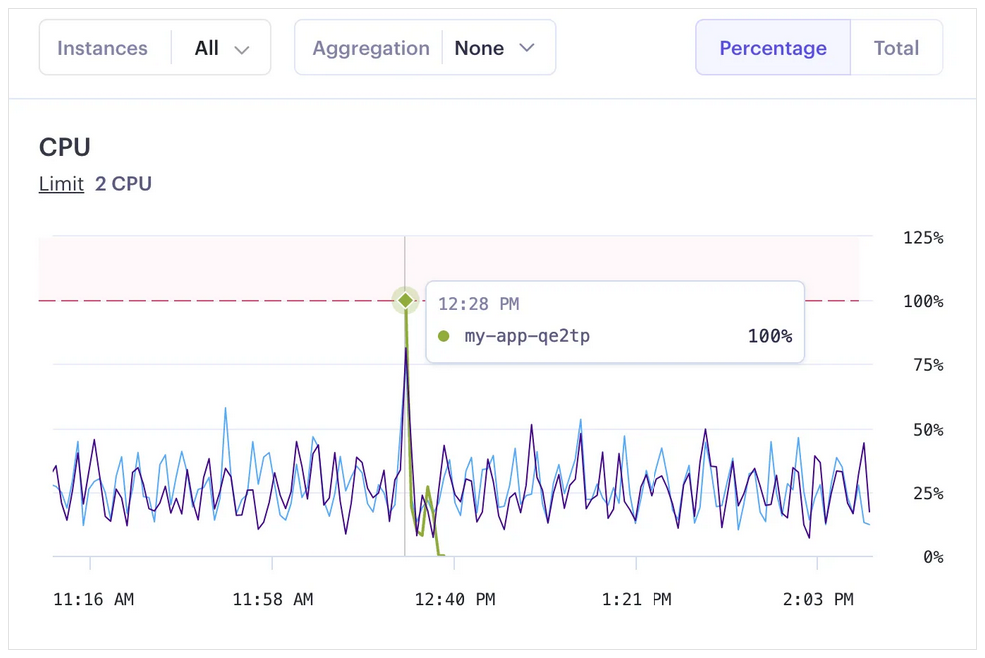
\includegraphics[width=0.50\linewidth]{assets/Ejemplo-metricas-Render1.png}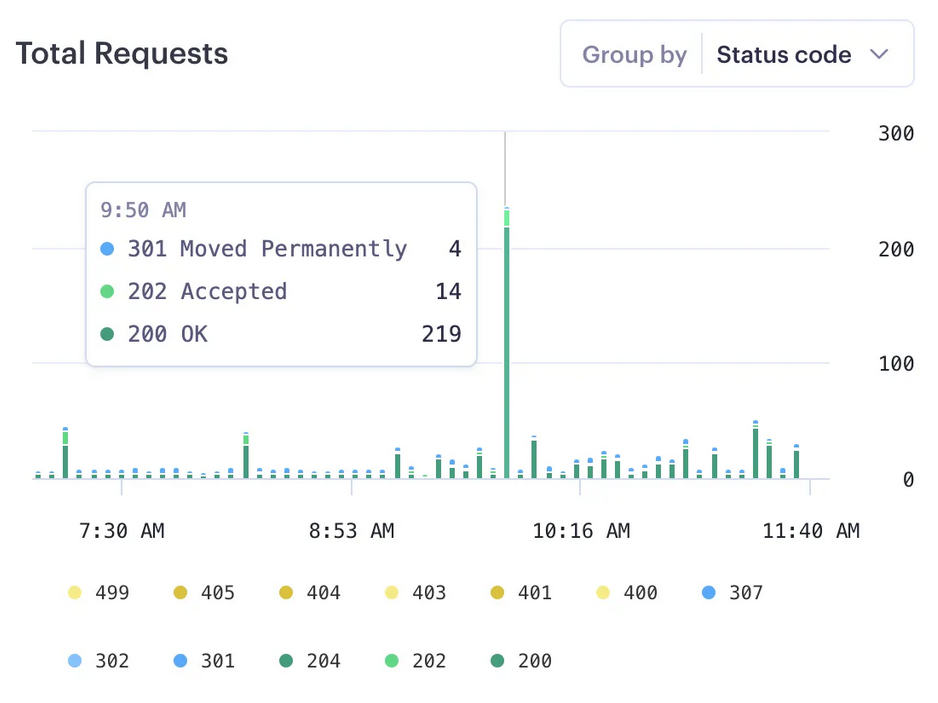
\includegraphics[width=0.50\linewidth]{assets/Ejemplo-metricas-Render2.png}
    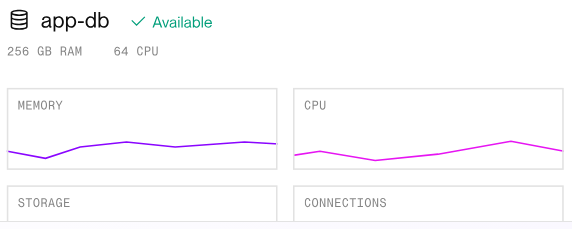
\includegraphics[width=0.50\linewidth]{assets/Ejemplo-metricas-Render3.png}
\end{figure}
\par
\vspace{5mm}

\subsubsection{Estimación de Coste para la Configuración Inicial}
A continuación se presenta la estimación de coste mensual para la
configuración con la que el sistema entrará en operación. Las cifras
están expresadas en dólares estadounidenses (USD), unidad de
facturación de Render, y se han verificado contra la tarifa pública del
proveedor en mayo de 2026.

\vspace{5mm}

\begin{longtable}[]{@{}
    % Metadatos de la tabla
        p{0.23\columnwidth}
        p{0.22\columnwidth}
        p{0.22\columnwidth}
        p{0.22\columnwidth}@{}}

    \caption{Coste para la Configuración Inicial} \\

    % Configuración de la tabla para repetir encabezados en cada página
    \toprule
    \textbf{Concepto} & \textbf{Plan} & \textbf{Características} & \textbf{Coste mensual} \\
    \midrule
    \endfirsthead % chktex 1

    \toprule
    \textbf{Concepto} & \textbf{Plan} & \textbf{Características} & \textbf{Coste mensual} \\
    \midrule
    \endhead % chktex 1

    \midrule
    \multicolumn{2}{r}{\small\emph{Continúa en la siguiente página}} \\
    \endfoot % chktex 1

    \bottomrule
    \endlastfoot % chktex 1

    % Cuerpo de la tabla
    Plan del workspace & Hobby & Gratuito, hasta 25 servicios, 5 GB de bandwidth, 
    copias de seguridad de 3 días & 0 USD \\
    \midrule

    Backend (Spring Boot) & Starter & 512 MB RAM, 0.5 CPU, sin hibernación & 7 USD \\
    \midrule

    Frontend (Angular) & Static Site & Servido desde CDN global, TLS automático & 0 USD \\
    \midrule

    Base de datos & PostgreSQL Basic-256mb & 256 MB RAM, 1 GB almacenamiento, 100 conexiones & 6 USD \\
    \midrule

    Dominio propio (.org / .es) & Anualidad prorrateada & Registro a través de proveedor externo & aprox. 1 USD \\ % chktex 26
    \midrule

    \textbf{Total estimado:} & & & \textbf{aprox. 14 USD/mes} \\
\end{longtable}

Considerar que dependiendo de la entidad bancaria, al momento de hacer\textbf{ el pago se puede cobrar una comisión por cambio 
de divisa}, lo que incrementaría el coste mensual.

\par
\vspace{5mm}

Este coste equivale aproximadamente a entre 13 y 15 EUR mensuales según
el tipo de cambio vigente. Es la configuración más eficiente compatible
con un funcionamiento continuo de producción, sin tiempos de espera al
acceder al sistema y con copias de seguridad automáticas de la base de
datos.


\subsubsection{Evolución Prevista del Coste}
A medida que el sistema gana adopción y la asociación afina su uso, el
coste mensual puede aumentar. La progresión razonable
prevista es la siguiente: meses 1 a 6 (desarrollo + primer período de uso) con el costo inicial (tabla anterior).
\par
\vspace{5mm} 
Luego ver como evoluciona en los meses 7 a 18 (operación con todo el voluntariado) para considerar migración del workspace 
al plan Pro con una base de datos a un nivel superior si hiciera falta (hasta 52 USD/mes). 
\par
\vspace{5mm}
Finalmente, a partir del año 2, 
si el uso se mantiene o crece, considerar ampliación de capacidad del backend (hasta 70 USD/mes) o limpieza de servicios 
no utilizados para optimizar costes o cambio de proveedor si el coste se vuelve insostenible.


\subsubsection{Modelo Económico del Producto}
El sistema es un desarrollo a medida sin modelo comercial asociado.
No se contempla su venta ni su licenciamiento a terceros en la versión
inicial. Si en el futuro otras asociaciones similares manifestaran
interés, podría evaluarse la liberación del código bajo licencia de
software libre o un modelo de servicio gestionado, pero esta decisión
queda fuera del alcance del presente documento.


\subsection{Estrategia de Mantenimiento}
Al ser una aplicación web, el usuario final no instala nada en su
dispositivo. El acceso al sistema se realiza mediante la dirección web
proporcionada por la asociación, abierta en el navegador de su
dispositivo al sitio web desplegado por Render.
\par
\vspace{5mm}
Las responsabilidades de despliegue y mantenimiento se
distribuyen como sigue:

\subsubsection*{Render asume:}
\begin{itemize}
    \item Provisión de la infraestructura física subyacente (servidores,
    almacenamiento, red).

    \item Mantenimiento del sistema operativo subyacente y parches de 
    seguridad de plataforma.

    \item Provisión y mantenimiento del servicio gestionado de PostgreSQL, 
    incluidas copias de seguridad diarias.

    \item Renovación automática del certificado TLS.\

    \item Monitorización de la salud básica del servicio (uptime, métricas de plataforma).

    \item Cifrado de las variables de entorno en reposo.
\end{itemize}


\subsubsection*{El equipo de desarrollo asume:}
\begin{itemize}
    \item Construcción y mantenimiento de las imágenes Docker.
    
    \item Configuración de los servicios en Render (variables de entorno,
    conexiones, escalado).

    \item Mantenimiento del pipeline de integración y despliegue continuos.
    
    \item Aplicación de actualizaciones de seguridad a las dependencias del proyecto.
    
    \item Implementación de copias de seguridad propias adicionales como redundancia.
    
    \item Monitorización aplicativa (logs, errores, métricas de negocio).
    
    \item Soporte funcional al usuario final.
\end{itemize}